
\kapitel{Continuous Integration}
To provide a continuous integration environment for this project Microsoft Azure DevOps was used.
\thispagestyle{plain}
\renewcommand\section{\stdsection}
\setcounter{section}{3}
\subsection{Microsoft Azure DevOps}
To use the ''Microsoft Azure DevOps'' a Microsoft account is required:
\\\\
\textbf{Microsoft Registration:} 
\\
\url{https://account.microsoft.com/account?lang=en-us}
\\\\
After the registration sign in ''Microsoft Azure DevOps'':
\\\\
\textbf{Microsoft Azure DevOps Sign-In:} 
\\
\url{https://dev.azure.com/}
\\\\
Use the following link to get started with ''Microsoft Azure DevOps'':
\\\\
\textbf{Getting Started with Microsoft Azure DevOps:} 
\\
\url{https://docs.microsoft.com/en-us/azure/devops/user-guide/sign-up-invite-teammates?view=vsts}

\subsubsection{Configuration}
There are some configurations to make for a minimal continuous integration with ''Microsoft Azure DevOps''. On the left hand side click on ''Pipelines - Builds'' and click on ''New Pipeline'':
\begin{figure}[H]
    \centering
    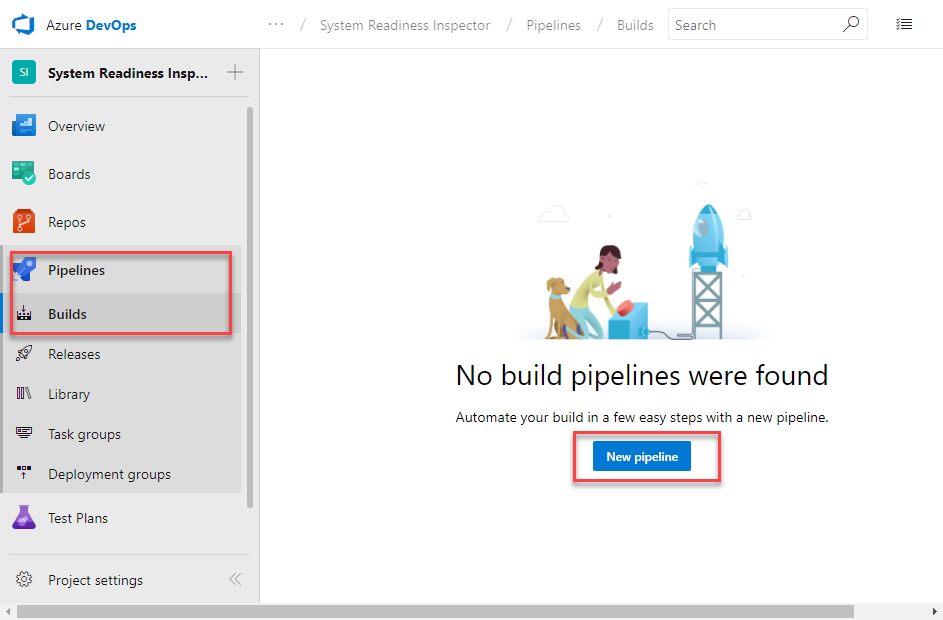
\includegraphics[width=0.7\linewidth]{../developer_manual/assets/devops1.png}
\end{figure}
Select your location of the source code. In this project GitHub was used:
\begin{figure}[H]
    \centering
    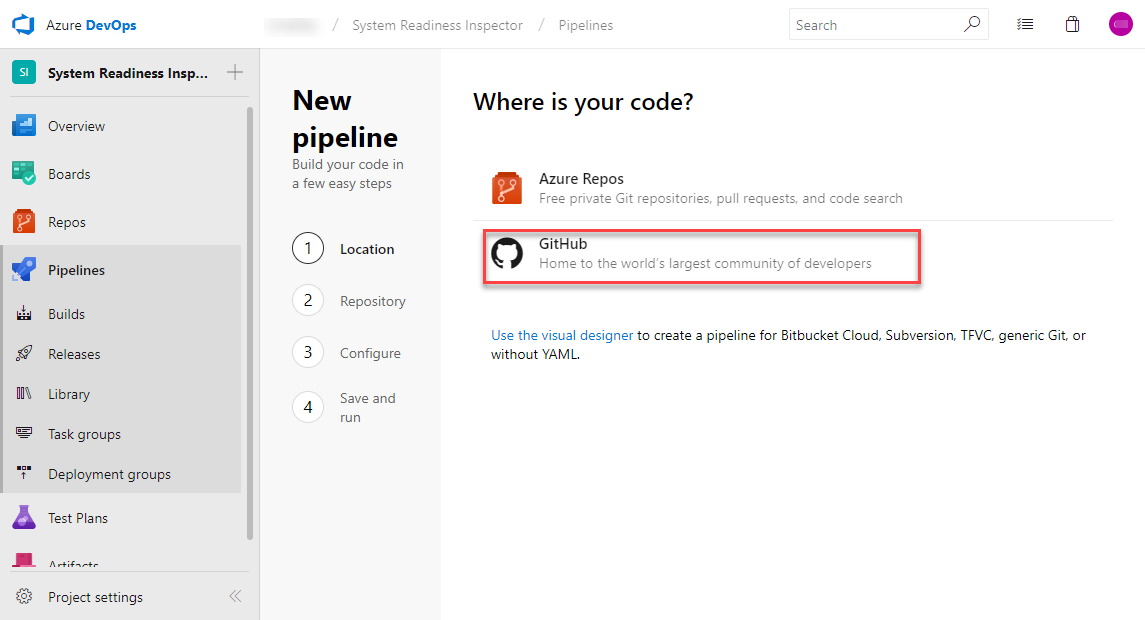
\includegraphics[width=0.7\linewidth]{../developer_manual/assets/devops2.png}
\end{figure}
After that, select your repository to use in your source code location:
\begin{figure}[H]
    \centering
    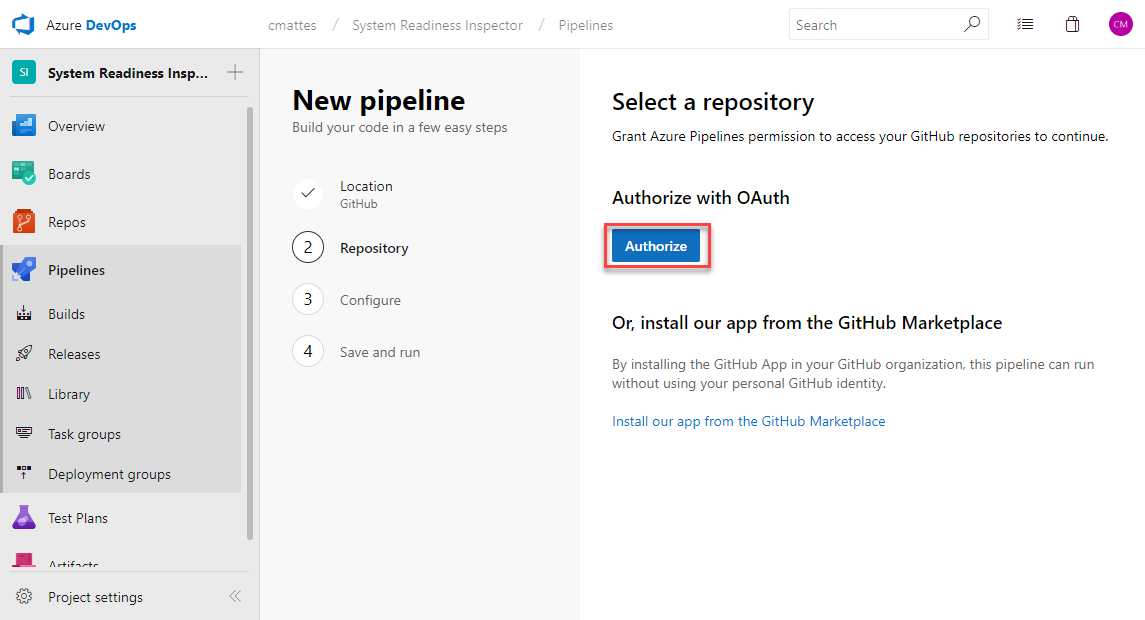
\includegraphics[width=0.7\linewidth]{../developer_manual/assets/devops3.png}
\end{figure}
Modify the YAML in the next step as provided after the printscreen and your continuous integration 

is ready to go:
\begin{figure}[H]
    \centering
    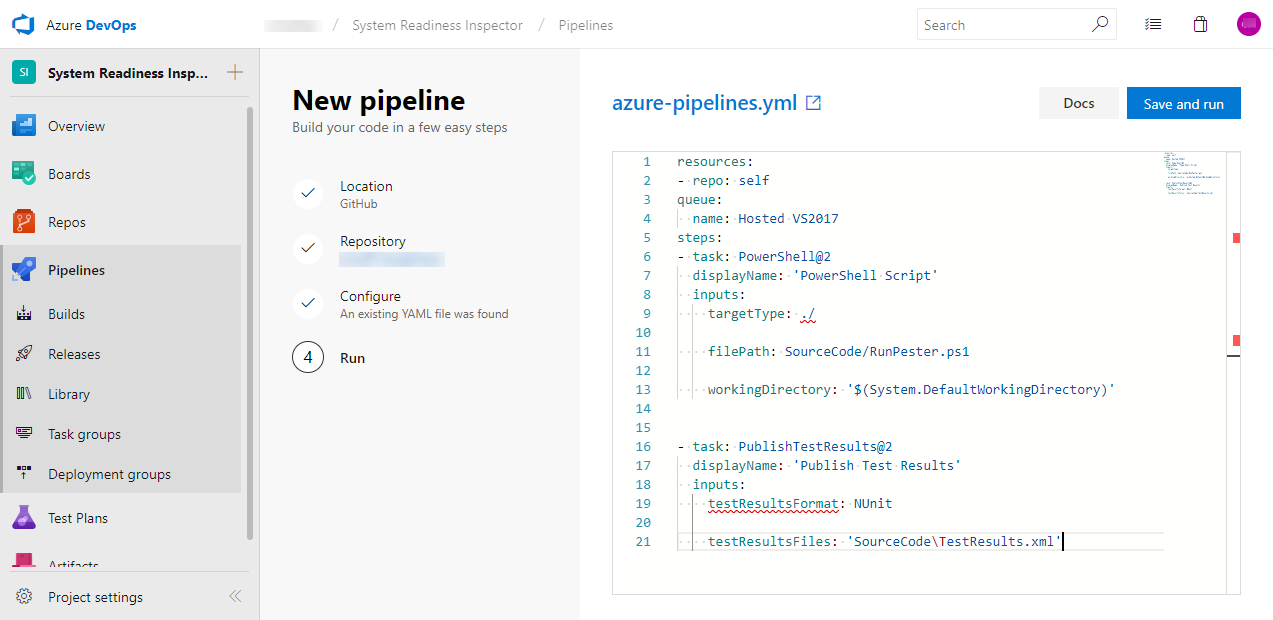
\includegraphics[width=0.7\linewidth]{../developer_manual/assets/devops4.png}
\end{figure}

\begin{lstlisting}
resources:
- repo: self
queue:
  name: Hosted VS2017
steps:
- task: PowerShell@2
  displayName: 'PowerShell Script'
  inputs:
    targetType: ./

    filePath: SourceCode/RunPester.ps1

    workingDirectory: '$(System.DefaultWorkingDirectory)'

- task: PublishTestResults@2
  displayName: 'Publish Test Results'
  inputs:
    testResultsFormat: NUnit

    testResultsFiles: 'SourceCode\TestResults.xml'
\end{lstlisting}\ \\
This YAML-File is adjusted for the use of the Pester test framework within the project. For more information use the following link, which provides additional information if needed:
\\
\url{https://www.powershellmagazine.com/2018/09/20/converting-a-powershell-project-to-use-azure-devops-pipelines/}